\documentclass{beamer}
\usepackage{physics}
\usepackage{amsmath}
\usepackage{tikz}
\usepackage{mathdots}
\usepackage{yhmath}
\usepackage{cancel}
\usepackage{color}
\usepackage{siunitx}
\usepackage{array}
\usepackage{multirow}
\usepackage{amssymb}
\usepackage{textcomp, gensymb}
\usepackage{tabularx}
\usepackage{extarrows}
\usepackage{booktabs}
\usetikzlibrary{fadings}
\usetikzlibrary{patterns}
\usetikzlibrary{shadows.blur}
\usetikzlibrary{shapes}
\usepackage[style=verbose,backend=bibtex]{biblatex}
\addbibresource{arpes.bib}
\addbibresource{green.bib}
\usepackage{listings}
\usepackage{hyperref}

\newcommand{\pair}[1]{\langle #1 \rangle}
\DeclareMathOperator{\ee}{e}
\DeclareMathOperator{\ii}{i}

\newcommand{\concept}[1]{\textbf{#1}}

%region Theme
\usetheme{Madrid}

% Show sectionin foot
\makeatletter
\setbeamertemplate{footline}
{
  \leavevmode%
  \hbox{%
  \begin{beamercolorbox}[wd=.333333\paperwidth,ht=2.25ex,dp=1ex,center]{author in head/foot}%
    \usebeamerfont{author in head/foot}\insertauthor
  \end{beamercolorbox}%
  \begin{beamercolorbox}[wd=.333333\paperwidth,ht=2.25ex,dp=1ex,center]{title in head/foot}%
    \usebeamerfont{title in head/foot}\insertsection
  \end{beamercolorbox}%
  \begin{beamercolorbox}[wd=.333333\paperwidth,ht=2.25ex,dp=1ex,right]{date in head/foot}%
    \usebeamerfont{date in head/foot}\insertshortdate{}\hspace*{2em}
    \insertframenumber{} / \inserttotalframenumber\hspace*{2ex} 
  \end{beamercolorbox}}%
  \vskip0pt%
}
\makeatother

%endregion

%Information to be included in the title page:
\title{Bosonic modes in Fermi liquid}
\author{Jinyuan Wu}

\begin{document}

\frame{\titlepage}

\section{Introduction}

\begin{frame}
\frametitle{Background}

In a Fermi liquid we have \dots
\begin{itemize}
    \item Quasiparticles (electron/hole) with $\Sigma$-correction
    \item Any anything else?
\end{itemize}    

\begin{center}
    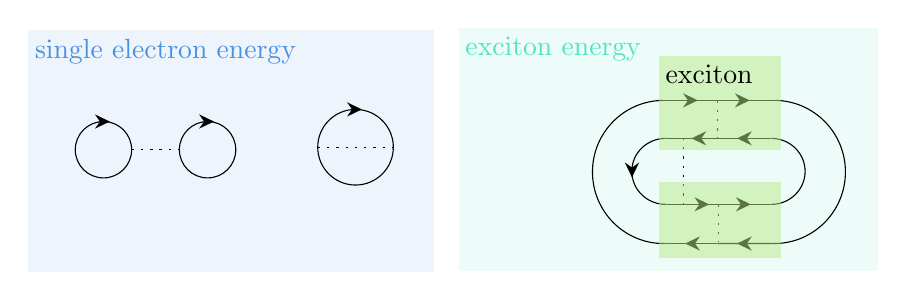
\begin{tikzpicture}[x=0.75pt,y=0.75pt,yscale=-1,xscale=1]
    %uncomment if require: \path (0,300); %set diagram left start at 0, and has height of 300
    
    %Shape: Rectangle [id:dp5146811729500922] 
    \draw  [draw opacity=0][fill={rgb, 255:red, 80; green, 227; blue, 194 }  ,fill opacity=0.1 ] (295.08,59.22) -- (497.25,59.22) -- (497.25,176.41) -- (295.08,176.41) -- cycle ;
    %Straight Lines [id:da6398455748193317] 
    \draw    (407.22,93.98) -- (407.28,93.98) ;
    \draw [shift={(410.28,93.98)}, rotate = 180] [fill={rgb, 255:red, 0; green, 0; blue, 0 }  ][line width=0.08]  [draw opacity=0] (7.14,-3.43) -- (0,0) -- (7.14,3.43) -- (4.74,0) -- cycle    ;
    %Straight Lines [id:da34436720244170616] 
    \draw    (393.72,93.98) -- (419.72,93.98) ;
    %Straight Lines [id:da5378870304376917] 
    \draw  [dash pattern={on 0.84pt off 2.51pt}]  (419.72,93.98) -- (419.72,112.28) ;
    %Straight Lines [id:da6880866744261185] 
    \draw    (432.22,93.98) -- (432.28,93.98) ;
    \draw [shift={(435.28,93.98)}, rotate = 180] [fill={rgb, 255:red, 0; green, 0; blue, 0 }  ][line width=0.08]  [draw opacity=0] (7.14,-3.43) -- (0,0) -- (7.14,3.43) -- (4.74,0) -- cycle    ;
    %Straight Lines [id:da08717980225255384] 
    \draw    (419.72,93.98) -- (447.27,93.98) ;
    %Straight Lines [id:da850721537949833] 
    \draw    (432.22,112.28) -- (432.17,112.28) ;
    \draw [shift={(429.17,112.28)}, rotate = 360] [fill={rgb, 255:red, 0; green, 0; blue, 0 }  ][line width=0.08]  [draw opacity=0] (7.14,-3.43) -- (0,0) -- (7.14,3.43) -- (4.74,0) -- cycle    ;
    %Straight Lines [id:da8852766962819558] 
    \draw    (445.72,112.28) -- (419.72,112.28) ;
    %Straight Lines [id:da2830293714598453] 
    \draw    (410.28,112.28) -- (410.22,112.28) ;
    \draw [shift={(407.22,112.28)}, rotate = 360] [fill={rgb, 255:red, 0; green, 0; blue, 0 }  ][line width=0.08]  [draw opacity=0] (7.14,-3.43) -- (0,0) -- (7.14,3.43) -- (4.74,0) -- cycle    ;
    %Straight Lines [id:da4409957948094987] 
    \draw    (419.72,112.28) -- (394.72,112.28) ;
    %Straight Lines [id:da166206845135215] 
    \draw    (378.56,127.98) -- (378.56,128.08) ;
    \draw [shift={(378.56,131.08)}, rotate = 270] [fill={rgb, 255:red, 0; green, 0; blue, 0 }  ][line width=0.08]  [draw opacity=0] (7.14,-3.43) -- (0,0) -- (7.14,3.43) -- (4.74,0) -- cycle    ;
    %Straight Lines [id:da8858104612113908] 
    \draw    (395.22,144.07) -- (420.22,144.07) ;
    %Straight Lines [id:da7115305058801602] 
    \draw  [dash pattern={on 0.84pt off 2.51pt}]  (420.22,144.07) -- (420.22,162.38) ;
    %Straight Lines [id:da4365031995623925] 
    \draw    (432.72,144.07) -- (432.77,144.07) ;
    \draw [shift={(435.77,144.07)}, rotate = 180] [fill={rgb, 255:red, 0; green, 0; blue, 0 }  ][line width=0.08]  [draw opacity=0] (7.14,-3.43) -- (0,0) -- (7.14,3.43) -- (4.74,0) -- cycle    ;
    %Straight Lines [id:da5381005184479546] 
    \draw    (420.22,144.07) -- (445.22,144.07) ;
    %Straight Lines [id:da5357673686633508] 
    \draw    (432.22,162.95) -- (432.17,162.95) ;
    \draw [shift={(429.17,162.95)}, rotate = 360] [fill={rgb, 255:red, 0; green, 0; blue, 0 }  ][line width=0.08]  [draw opacity=0] (7.14,-3.43) -- (0,0) -- (7.14,3.43) -- (4.74,0) -- cycle    ;
    %Straight Lines [id:da7809394137927026] 
    \draw    (446.19,162.94) -- (419.72,162.95) ;
    %Straight Lines [id:da0014751437976323611] 
    \draw    (407.22,162.95) -- (407.17,162.95) ;
    \draw [shift={(404.17,162.95)}, rotate = 360] [fill={rgb, 255:red, 0; green, 0; blue, 0 }  ][line width=0.08]  [draw opacity=0] (7.14,-3.43) -- (0,0) -- (7.14,3.43) -- (4.74,0) -- cycle    ;
    %Straight Lines [id:da4139281131726549] 
    \draw    (419.72,162.95) -- (394.72,162.95) ;
    %Shape: Arc [id:dp842942564916912] 
    \draw  [draw opacity=0] (395.22,144.07) .. controls (395.08,144.07) and (394.95,144.08) .. (394.81,144.08) .. controls (385.78,144.08) and (378.47,136.96) .. (378.47,128.18) .. controls (378.47,119.43) and (385.74,112.33) .. (394.72,112.28) -- (394.81,128.18) -- cycle ; \draw   (395.22,144.07) .. controls (395.08,144.07) and (394.95,144.08) .. (394.81,144.08) .. controls (385.78,144.08) and (378.47,136.96) .. (378.47,128.18) .. controls (378.47,119.43) and (385.74,112.33) .. (394.72,112.28) ;  
    %Straight Lines [id:da7052800705155782] 
    \draw  [dash pattern={on 0.84pt off 2.51pt}]  (403.39,111.98) -- (403.39,143.41) ;
    %Straight Lines [id:da7494886948705168] 
    \draw    (412.72,144.07) -- (412.77,144.07) ;
    \draw [shift={(415.77,144.07)}, rotate = 180] [fill={rgb, 255:red, 0; green, 0; blue, 0 }  ][line width=0.08]  [draw opacity=0] (7.14,-3.43) -- (0,0) -- (7.14,3.43) -- (4.74,0) -- cycle    ;
    %Shape: Arc [id:dp6452390768047809] 
    \draw  [draw opacity=0] (445.22,144.07) .. controls (445.36,144.07) and (445.49,144.08) .. (445.63,144.08) .. controls (454.65,144.08) and (461.97,136.96) .. (461.97,128.18) .. controls (461.97,119.43) and (454.7,112.33) .. (445.72,112.28) -- (445.63,128.18) -- cycle ; \draw   (445.22,144.07) .. controls (445.36,144.07) and (445.49,144.08) .. (445.63,144.08) .. controls (454.65,144.08) and (461.97,136.96) .. (461.97,128.18) .. controls (461.97,119.43) and (454.7,112.33) .. (445.72,112.28) ;  
    %Shape: Arc [id:dp43945222094751113] 
    \draw  [draw opacity=0] (446.19,162.94) .. controls (446.49,162.95) and (446.78,162.95) .. (447.08,162.95) .. controls (466.03,162.95) and (481.39,147.51) .. (481.39,128.46) .. controls (481.39,109.48) and (466.13,94.08) .. (447.27,93.98) -- (447.08,128.46) -- cycle ; \draw   (446.19,162.94) .. controls (446.49,162.95) and (446.78,162.95) .. (447.08,162.95) .. controls (466.03,162.95) and (481.39,147.51) .. (481.39,128.46) .. controls (481.39,109.48) and (466.13,94.08) .. (447.27,93.98) ;  
    %Shape: Arc [id:dp9293716217993426] 
    \draw  [draw opacity=0] (394.72,162.95) .. controls (394.43,162.96) and (394.13,162.96) .. (393.83,162.96) .. controls (374.88,162.96) and (359.52,147.52) .. (359.52,128.47) .. controls (359.52,109.49) and (374.78,94.09) .. (393.64,93.99) -- (393.83,128.47) -- cycle ; \draw   (394.72,162.95) .. controls (394.43,162.96) and (394.13,162.96) .. (393.83,162.96) .. controls (374.88,162.96) and (359.52,147.52) .. (359.52,128.47) .. controls (359.52,109.49) and (374.78,94.09) .. (393.64,93.99) ;  
    %Shape: Rectangle [id:dp7966285154601207] 
    \draw  [draw opacity=0][fill={rgb, 255:red, 184; green, 233; blue, 134 }  ,fill opacity=0.5 ] (391.5,72.52) -- (450.5,72.52) -- (450.5,117.67) -- (391.5,117.67) -- cycle ;
    %Shape: Rectangle [id:dp15539312444775466] 
    \draw  [draw opacity=0][fill={rgb, 255:red, 184; green, 233; blue, 134 }  ,fill opacity=0.5 ] (391.5,133.52) -- (450.5,133.52) -- (450.5,169.81) -- (391.5,169.81) -- cycle ;
    
    %Shape: Rectangle [id:dp27994217946502586] 
    \draw  [draw opacity=0][fill={rgb, 255:red, 74; green, 144; blue, 226 }  ,fill opacity=0.1 ] (87.67,60.09) -- (283.39,60.09) -- (283.39,176.85) -- (87.67,176.85) -- cycle ;
    %Shape: Circle [id:dp462236419122503] 
    \draw   (110.33,117.75) .. controls (110.33,110.25) and (116.41,104.17) .. (123.92,104.17) .. controls (131.42,104.17) and (137.5,110.25) .. (137.5,117.75) .. controls (137.5,125.25) and (131.42,131.33) .. (123.92,131.33) .. controls (116.41,131.33) and (110.33,125.25) .. (110.33,117.75) -- cycle ;
    %Straight Lines [id:da670513630425587] 
    \draw  [dash pattern={on 0.84pt off 2.51pt}]  (137.5,117.75) -- (160.5,117.75) ;
    %Shape: Circle [id:dp7720535201865808] 
    \draw   (160.5,117.75) .. controls (160.5,110.25) and (166.58,104.17) .. (174.08,104.17) .. controls (181.59,104.17) and (187.67,110.25) .. (187.67,117.75) .. controls (187.67,125.25) and (181.59,131.33) .. (174.08,131.33) .. controls (166.58,131.33) and (160.5,125.25) .. (160.5,117.75) -- cycle ;
    %Straight Lines [id:da8207419794627446] 
    \draw    (174.08,104.17) -- (174.14,104.17) ;
    \draw [shift={(177.14,104.17)}, rotate = 180] [fill={rgb, 255:red, 0; green, 0; blue, 0 }  ][line width=0.08]  [draw opacity=0] (7.14,-3.43) -- (0,0) -- (7.14,3.43) -- (4.74,0) -- cycle    ;
    %Straight Lines [id:da15224804787584634] 
    \draw    (123.92,104.17) -- (123.97,104.17) ;
    \draw [shift={(126.97,104.17)}, rotate = 180] [fill={rgb, 255:red, 0; green, 0; blue, 0 }  ][line width=0.08]  [draw opacity=0] (7.14,-3.43) -- (0,0) -- (7.14,3.43) -- (4.74,0) -- cycle    ;
    
    %Shape: Circle [id:dp2405384911845121] 
    \draw   (227.15,116.55) .. controls (227.15,106.49) and (235.3,98.33) .. (245.36,98.33) .. controls (255.43,98.33) and (263.58,106.49) .. (263.58,116.55) .. controls (263.58,126.61) and (255.43,134.77) .. (245.36,134.77) .. controls (235.3,134.77) and (227.15,126.61) .. (227.15,116.55) -- cycle ;
    %Straight Lines [id:da004084517255771747] 
    \draw  [dash pattern={on 0.84pt off 2.51pt}]  (227.15,116.55) -- (236.71,116.55) -- (263.58,116.55) ;
    %Straight Lines [id:da2452546368901709] 
    \draw    (245.36,98.33) -- (245.42,98.33) ;
    \draw [shift={(248.42,98.33)}, rotate = 180] [fill={rgb, 255:red, 0; green, 0; blue, 0 }  ][line width=0.08]  [draw opacity=0] (7.14,-3.43) -- (0,0) -- (7.14,3.43) -- (4.74,0) -- cycle    ;
    
    
    % Text Node
    \draw (89.67,63.09) node [anchor=north west][inner sep=0.75pt]  [color={rgb, 255:red, 74; green, 144; blue, 226 }  ,opacity=1 ] [align=left] {single electron energy};
    % Text Node
    \draw (393.5,75.52) node [anchor=north west][inner sep=0.75pt]   [align=left] {exciton};
    % Text Node
    \draw (297.08,62.22) node [anchor=north west][inner sep=0.75pt]  [color={rgb, 255:red, 80; green, 227; blue, 194 }  ,opacity=1 ] [align=left] {exciton energy};
    
    
    \end{tikzpicture}
    
\end{center}

\dots and more

\end{frame}

\begin{frame}
\frametitle{Question}

\onslide<1->{
    \textbf{What to do}

    Finding modes other than the corrected single electron/hole   
    
    \vspace{0.6cm}

    \textbf{Why it's important} 
    
    Usually not for $C_V$ but for optical response: $\epsilon$, $\chi^{(3)}$, etc.
}

\onslide<2->{
    \vspace{0.6cm}

    \textbf{Today's topic}

    Electron-hole bosonic modes in Fermi liquid 
    (with \emph{some} scattering picked up back, i.e. 
    beyond $\var{E} \sim \varepsilon \var{n} + f \var{n} \var{n}$), i.e.
    \begin{equation}
        \protect\ket*{\text{single excitation}} = \sum _{\boldsymbol{k}_{1} ,\boldsymbol{k}_{2}} c_{\boldsymbol{k}_{1}\boldsymbol{k}_{2}}\ket{\tikzset{every picture/.style={line width=0.75pt}} %set default line width to 0.75pt        
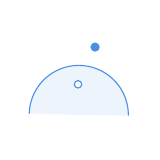
\begin{tikzpicture}[x=0.75pt,y=0.75pt,yscale=-0.5,xscale=0.5, baseline=(XXXX.south) ]
\path (0,100);\path (100,0);\draw    ($(current bounding box.center)+(0,0.3em)$) node [anchor=south] (XXXX) {};
%Shape: Arc [id:dp8520886122690758] 
\draw  [draw opacity=0][fill={rgb, 255:red, 74; green, 144; blue, 226 }  ,fill opacity=0.1 ] (1.48,82.71) .. controls (1.97,66.38) and (10.83,50.73) .. (26.17,42.28) .. controls (49.27,29.54) and (78.33,37.94) .. (91.06,61.04) .. controls (95.22,68.59) and (97.13,76.77) .. (97,84.81) -- (49.23,84.11) -- cycle ; \draw  [color={rgb, 255:red, 74; green, 144; blue, 226 }  ,draw opacity=1 ] (1.48,82.71) .. controls (1.97,66.38) and (10.83,50.73) .. (26.17,42.28) .. controls (49.27,29.54) and (78.33,37.94) .. (91.06,61.04) .. controls (95.22,68.59) and (97.13,76.77) .. (97,84.81) ;  
%Straight Lines [id:da9414882934326914] 
\draw [color={rgb, 255:red, 74; green, 144; blue, 226 }  ,draw opacity=1 ]   (64.93,18.71) ;
\draw [shift={(64.93,18.71)}, rotate = 0] [color={rgb, 255:red, 74; green, 144; blue, 226 }  ,draw opacity=1 ][fill={rgb, 255:red, 74; green, 144; blue, 226 }  ,fill opacity=1 ][line width=0.75]      (0, 0) circle [x radius= 3.35, y radius= 3.35]   ;
%Shape: Circle [id:dp32914036484275444] 
\draw  [color={rgb, 255:red, 74; green, 144; blue, 226 }  ,draw opacity=1 ][fill={rgb, 255:red, 255; green, 255; blue, 255 }  ,fill opacity=1 ] (44.93,54.6) .. controls (44.93,52.62) and (46.53,51.01) .. (48.51,51.01) .. controls (50.49,51.01) and (52.1,52.62) .. (52.1,54.6) .. controls (52.1,56.58) and (50.49,58.18) .. (48.51,58.18) .. controls (46.53,58.18) and (44.93,56.58) .. (44.93,54.6) -- cycle ;
\end{tikzpicture}
}
    \end{equation}

    No trion, higher order correlation, or even more exotic spinons, etc. beyond Fermi liquid
}

\end{frame}


\begin{frame}
\frametitle{Overview}

Three types of important bosonic modes:

\begin{itemize}
    \item Zero sound in uncharged single-band Fermi liquid
    \item Plasmon in charged single-band Fermi liquid = zero sound + long range interaction 
    \item Exciton in charged multi-band Fermi liquid
\end{itemize}

\end{frame}

\begin{frame}
\frametitle{Methodology}

\textbf{Series calculation} 

Bethe–Salpeter equation (BSE) is used for quantitative calculations. 

\emph{Problem}: no picture about ``how the electron moves''

\vspace{0.5cm}

\textbf{Linking BSE with single-electron picture}

Linear response of single-electron under external field = BSE

\vspace{0.5cm}

\textbf{Simplified response theory}

We use quantum Boltzmann equation (QBE)



\end{frame}

\section{Discussion}

\begin{frame}
\frametitle{Discussion}

\textbf{Is QBE reliable?}

\emph{Yes!} When we intuitively expect it to work --

\begin{center}
    

\tikzset{every picture/.style={line width=0.75pt}} %set default line width to 0.75pt        

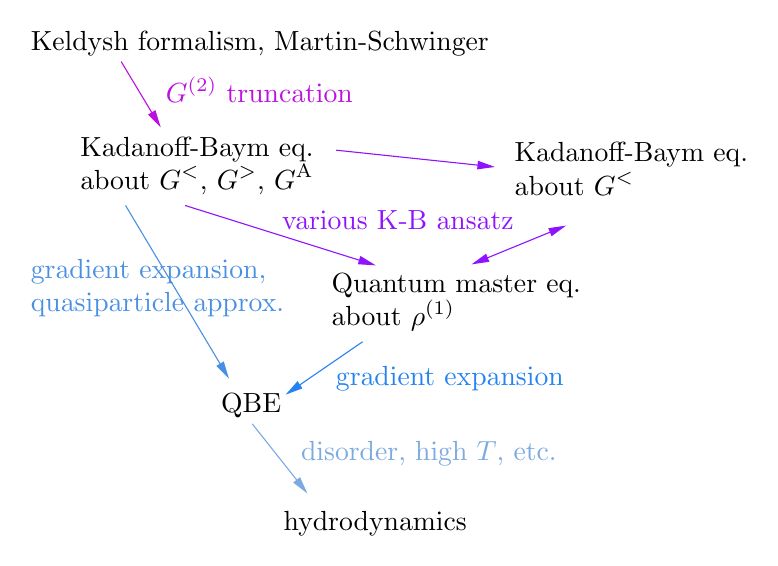
\begin{tikzpicture}[x=0.75pt,y=0.75pt,yscale=-0.7,xscale=0.7]
%uncomment if require: \path (0,409); %set diagram left start at 0, and has height of 409

%Straight Lines [id:da9993448313111608] 
\draw [color={rgb, 255:red, 189; green, 16; blue, 224 }  ,draw opacity=1 ]   (100,52) -- (126.14,95.47) ;
\draw [shift={(127.17,97.19)}, rotate = 238.99] [fill={rgb, 255:red, 189; green, 16; blue, 224 }  ,fill opacity=1 ][line width=0.08]  [draw opacity=0] (12,-3) -- (0,0) -- (12,3) -- cycle    ;
%Straight Lines [id:da505450204640074] 
\draw [color={rgb, 255:red, 144; green, 19; blue, 254 }  ,draw opacity=1 ]   (144,151) -- (273.26,191.59) ;
\draw [shift={(275.17,192.19)}, rotate = 197.43] [fill={rgb, 255:red, 144; green, 19; blue, 254 }  ,fill opacity=1 ][line width=0.08]  [draw opacity=0] (12,-3) -- (0,0) -- (12,3) -- cycle    ;
%Straight Lines [id:da7259646168352232] 
\draw [color={rgb, 255:red, 74; green, 144; blue, 226 }  ,draw opacity=1 ]   (103,151) -- (173.14,268.47) ;
\draw [shift={(174.17,270.19)}, rotate = 239.16] [fill={rgb, 255:red, 74; green, 144; blue, 226 }  ,fill opacity=1 ][line width=0.08]  [draw opacity=0] (12,-3) -- (0,0) -- (12,3) -- cycle    ;
%Straight Lines [id:da35768014069365206] 
\draw [color={rgb, 255:red, 36; green, 131; blue, 241 }  ,draw opacity=1 ]   (266.17,244.78) -- (214.82,280.06) ;
\draw [shift={(213.17,281.19)}, rotate = 325.51] [fill={rgb, 255:red, 36; green, 131; blue, 241 }  ,fill opacity=1 ][line width=0.08]  [draw opacity=0] (12,-3) -- (0,0) -- (12,3) -- cycle    ;
%Straight Lines [id:da15985835431985884] 
\draw [color={rgb, 255:red, 124; green, 170; blue, 224 }  ,draw opacity=1 ]   (190.17,301.25) -- (226.93,347.68) ;
\draw [shift={(228.17,349.25)}, rotate = 231.63] [fill={rgb, 255:red, 124; green, 170; blue, 224 }  ,fill opacity=1 ][line width=0.08]  [draw opacity=0] (12,-3) -- (0,0) -- (12,3) -- cycle    ;
%Straight Lines [id:da33183770683384806] 
\draw [color={rgb, 255:red, 144; green, 19; blue, 254 }  ,draw opacity=1 ]   (248,112.94) -- (355.18,124.25) ;
\draw [shift={(357.17,124.46)}, rotate = 186.02] [fill={rgb, 255:red, 144; green, 19; blue, 254 }  ,fill opacity=1 ][line width=0.08]  [draw opacity=0] (12,-3) -- (0,0) -- (12,3) -- cycle    ;
%Straight Lines [id:da43680180859475204] 
\draw [color={rgb, 255:red, 144; green, 19; blue, 254 }  ,draw opacity=1 ]   (404.32,165.61) -- (343.02,190.76) ;
\draw [shift={(341.17,191.52)}, rotate = 337.69] [fill={rgb, 255:red, 144; green, 19; blue, 254 }  ,fill opacity=1 ][line width=0.08]  [draw opacity=0] (12,-3) -- (0,0) -- (12,3) -- cycle    ;
\draw [shift={(406.17,164.85)}, rotate = 157.69] [fill={rgb, 255:red, 144; green, 19; blue, 254 }  ,fill opacity=1 ][line width=0.08]  [draw opacity=0] (12,-3) -- (0,0) -- (12,3) -- cycle    ;

% Text Node
\draw (36,29) node [anchor=north west][inner sep=0.75pt]   [align=left] {Keldysh formalism, Martin-Schwinger};
% Text Node
\draw (195.1,71.44) node  [color={rgb, 255:red, 189; green, 16; blue, 224 }  ,opacity=1 ] [align=left] {$\displaystyle G^{( 2)}$ truncation};
% Text Node
\draw (70,102) node [anchor=north west][inner sep=0.75pt]   [align=left] {Kadanoff-Baym eq.\\about $\displaystyle G^{< }$, $\displaystyle G^{ >}$, $\displaystyle G^{\text{A}}$};
% Text Node
\draw (209,153) node [anchor=north west][inner sep=0.75pt]  [color={rgb, 255:red, 144; green, 19; blue, 254 }  ,opacity=1 ] [align=left] {various K-B ansatz};
% Text Node
\draw (243,196) node [anchor=north west][inner sep=0.75pt]   [align=left] {Quantum master eq.\\about $\displaystyle \rho ^{( 1)}$};
% Text Node
\draw (36,186) node [anchor=north west][inner sep=0.75pt]  [color={rgb, 255:red, 74; green, 144; blue, 226 }  ,opacity=1 ] [align=left] {gradient expansion,\\quasiparticle approx.};
% Text Node
\draw (167,279) node [anchor=north west][inner sep=0.75pt]   [align=left] {QBE};
% Text Node
\draw (246,260) node [anchor=north west][inner sep=0.75pt]  [color={rgb, 255:red, 36; green, 131; blue, 241 }  ,opacity=1 ] [align=left] {gradient expansion};
% Text Node
\draw (222,311.45) node [anchor=north west][inner sep=0.75pt]  [color={rgb, 255:red, 124; green, 170; blue, 224 }  ,opacity=1 ] [align=left] {disorder, high $\displaystyle T$, etc.};
% Text Node
\draw (210,359.45) node [anchor=north west][inner sep=0.75pt]   [align=left] {hydrodynamics};
% Text Node
\draw (369,106) node [anchor=north west][inner sep=0.75pt]   [align=left] {Kadanoff-Baym eq.\\about $\displaystyle G^{< }$};


\end{tikzpicture}

\end{center}

\end{frame}

\begin{frame}
\frametitle{Discussion}



\end{frame}

\end{document}